\chapter{Methods for solving QUBO problems}\label{review}
\vspace{2em}

This chapter reviews the different approaches used to solve QUBO problems, which are broadly categorised as Classical, Quantum Annealing, Neural Network Quantum States, and Hybrid Quantum-Classical Algorithms.

\section{Classical}
Classical approaches search for solutions to QUBO problems without exploiting quantum properties. A typical classical approach is by exact diagonalisation of the corresponding Ising Hamiltonian~\cite{b25}. Exact diagonalisation solves for all the eigenvalues and eigenvectors and is also known as eigendecomposition, which is always possible for quantum Hamiltonians as they are represented by Hermitian matrices~\cite{b27}. However, the runtime of exact diagonalisation scales exponentially with input problem size and becomes computationally infeasible once the matrix grows large \cite{b25}. Since we are only interested in finding the smallest eigenvalue and the corresponding eigenvector, we can use iterative methods such as the Lanczos algorithm \cite{b28} or the implicitly restarted Arnoldi method \cite{b29} to find the smallest eigenvalue. However, such methods often run into stability issues. There are also branch and bound methods for solving QUBO problems, which aim to repeatedly break down the QUBO problem into subproblems and build lower and upper bounds for the objective values of the subproblems \cite{otaki2023experimental}. However, such methods might only work well for specific classes of problems and may not apply to a general QUBO problem.

Due to the exponentially increasing search space, some classical methods aim to find approximate solutions to QUBO problems instead. One class of approximate methods relies on heuristics to search for optimal solutions. \outcite{b12} systematically reviewed and evaluated published heuristics for QUBO problems. However, heuristics often only work well for a certain type of QUBO problems and do not generalise well.

%For example, variants of Tabu search---a local search algorithm that allows for moves that are not improvements and discourages visiting already visited states---are highly competitive heuristic algorithms to find good solutions to QUBO problems\cite{b2,b30}. 

Another approximate method for solving QUBO problems is simulated annealing. Simulated annealing \cite{Kirkpatrick} is a probabilistic method that starts with an initial trial state and a temperature $T$, which decreases slowly during the search. In each iteration, the algorithm samples neighbouring states of the current state and accepts the new sample based on the difference in energy, $\Delta E$, between the current state and the new state. If $\Delta E < 0$, the new sample is always accepted, and if $\Delta E \geq 0$, the new sample is accepted with probability $\propto e^{-\frac{\Delta E}{T}}$. The algorithm to sample new states is adapted from the Metropolis-Hastings sampling method \cite{metropolissampling}, and the chance to explore poorer solutions allows the algorithm to escape local minima and find the global minima in the limit of infinite annealing time.

For the motivated reader, \outcite{punnen2022quadratic} conducted a detailed survey of classical methods for solving QUBO problems.

\section{Quantum Annealing}\label{section:annealing}
Quantum annealing, introduced by \outcite{kadowaki1998quantum}, is used to find the ground state configuration of Ising models. To solve a QUBO problem with quantum annealing, we first convert it to the equivalent Ising model and then use the \textit{adiabatic theorem} to find its ground state configuration. The \textit{adiabatic theorem} states that "a quantum system in its ground state will remain in the ground state, provided that the Hamiltonian governing the dynamics changes sufficiently slowly" \cite{b15}. If we can manipulate the final Hamiltonian of a quantum system to one that describes the Ising model of interest, then we can find the ground state of the Ising model simply by measuring the final configuration of the quantum system.

%\begin{figure}[htb!]
%    \centering
%    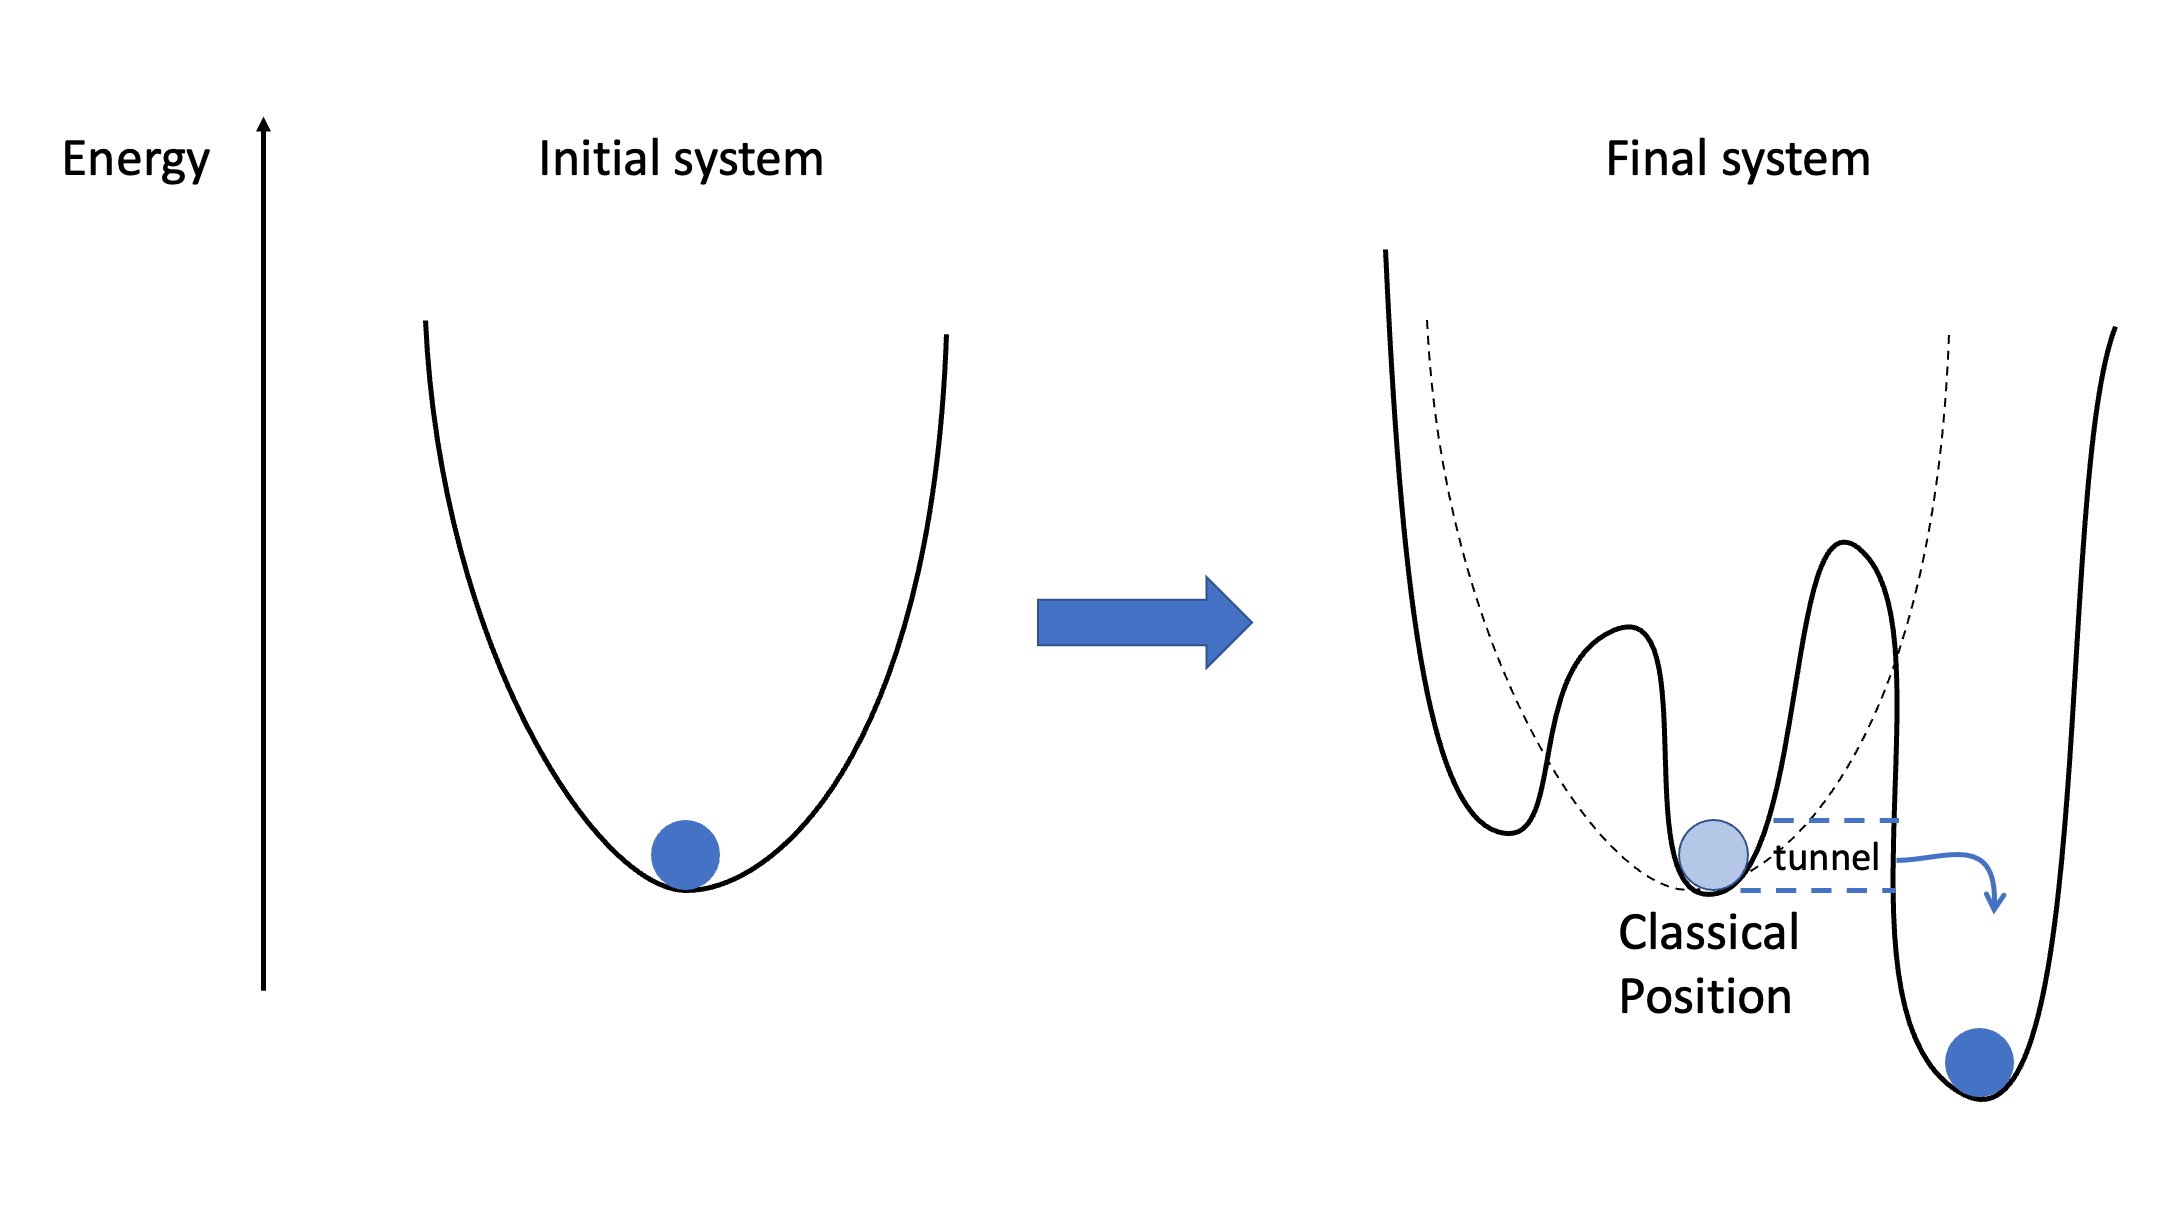
\includegraphics[width=0.8\linewidth]{images/quantum_annealing.png}
%    \caption{Energy landscape before (left) and after (right) quantum annealing}
%    \label{quantumannealing}
%\end{figure}
Quantum annealers first prepare a system in the ground state with a simple initial Hamiltonian $H_0$ (called the mixer or tunnelling Hamiltonian), with a simple energy landscape. Then, the system Hamiltonian is slowly changed to a more complex form $H_c$ \cite{b10}, with a complex energy landscape. The Hamiltonian at any point $H(s)$ can be written as
\begin{equation}
    \label{eqn:annealinghamiltonian}
    H(s) = A(s)H_0 + B(s)H_c
\end{equation}
where $s \in [0,1]$ is the normalised anneal fraction and $A(s)$ and $B(s)$ are decreasing and increasing functions. At the start of the annealing, we should have $A(s) >> B(s)$, and at the end of the annealing, we should have $B(s) >> A(s)$. If the transition time is sufficiently large, the adiabatic theorem ensures that the system will remain in the ground state, which can then be measured to yield the desired ground state configuration of $H_c$ \cite{b14}.

As $H_0$ usually consists of interactions terms with a transverse magnetic field and does not commute with the target Hamiltonian $H_c$, it allows for quantum tunnelling through energy barriers between classical states \cite{kadowaki1998quantum}. Quantum tunnelling allows the wave function to remain at the ground state even when classical search methods may end up stuck in a local minimum. However, the adiabatic theorem requires an arbitrarily long anneal time to guarantee that the system remains in the ground state, which is not feasible for practical purposes. Current implementations of quantum annealing instead rely on a finite time annealing with repeated sampling to increase the probability of finding the ground state \abbrevcite{farhi2001}.

Quantum annealing has been extensively studied and applied to solve various types of combinatorial optimisation problems, such as scheduling \abbrevcite{b17}, portfolio optimisation \abbrevcite{b18}, and quantum simulations \abbrevcite{b19}. There are also significant roadblocks in scaling the currently limited hardware capabilities \cite{b14}, and debate on whether quantum annealing will eventually run faster than classical search methods \cite{b10}. However, there is hope that these challenges can be mitigated in the near future with the rapid progress in quantum computing technology. D-Wave Systems, a Canadian-based quantum computing company, is the current leading commercial provider of quantum annealing hardware \cite{b16}.

\section{Neural-Network Quantum States}
\outcite{b20} introduced a neural-network-based method for approximating the wave function of a target quantum system with an artificial neural network as \textit{neural-network quantum states} (NNQS). The authors used the method to find the ground state and time evolution of the Ising and Heisenberg models in Physics. The NNQS is used as an Ansatz to approximate the wave function, which can be viewed as a probability distribution over the possible system configurations \cite{b25}.

The theoretical foundations for NNQS's ability to approximate wave functions rely on the \textit{Kolmogorov-Arnold representation theorem} \cite{kolmogorov1957representation}, which implies that neural networks can represent all multivariate, smooth functions. Since the wave function generally satisfies these requirements, we can expect that a neural network can reasonably approximate the wave function of a quantum system \cite{b20}.

The original NNQS architecture utilised a Restricted Boltzmann Machine (RBM) as its underlying neural network \cite{b20}. The RBM, shown in \autoref{rbmstructure}, is an energy-based generative model that has three components: a visible layer $\boldsymbol{s}$ with $n$ nodes, a hidden layer $\boldsymbol{h}$ with $m$ nodes, and a weight matrix $\mathbf{W}$. The number of hidden nodes is generally a multiple of the number of visible nodes, and the ratio $\alpha = \frac{m}{n}$ is a hyperparameter of the model. Each visible node $s_i$ is connected to every hidden node $h_j$ with a certain weight $W_{ij}$, but there are no connections within the visible or hidden layer. In other words, the visible and hidden nodes of the RBM form a bipartite graph.
\begin{figure}[htb!]
    \centering
    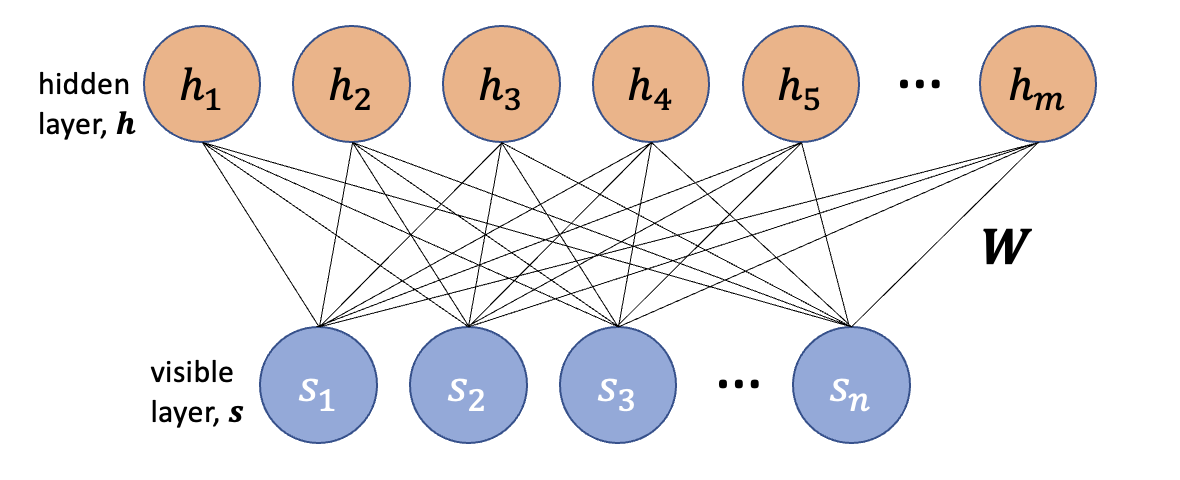
\includegraphics[width=0.7\linewidth]{images/rbm_diagram.png}
    \caption{Structure of a Restricted Boltzmann Machine}
    \label{rbmstructure}
\end{figure}

When approximating the wave function of an Ising model, each visible node $s_i$ represents the spin of a particle in the Ising model and can only take on the values of $1$ and $-1$ \cite{b20}. The representation of the wave function by the RBM can be expressed as:
\begin{equation}
    \Hat{\Psi}(\boldsymbol{s} ; \boldsymbol{\theta}_{rbm}) = \sum_{h} e^{\sum_i a_s s_i + \sum_j b_j h_j + \sum_{i,j}W_i s_i h_j} 
\end{equation}
where $\boldsymbol{\theta}_{rbm} = \{\boldsymbol{a}, \boldsymbol{b}, \boldsymbol{W}\}$ are the biases and weights of the RBM \cite{b20}. The network weights $\mathbf{W}$ are usually updated by performing Gibbs sampling, calculating the average energy of sampled configurations, and using either gradient-based optimisers or the stochastic reconfiguration method to derive the weight updates \cite{b25}.

Other neural network architectures, such as the Multilayer Perceptron (MLP), can also be used for NNQS. The MLP is a feedforward artificial neural network that consists of an input layer $\boldsymbol{x}$, one or more hidden layers, and an output layer. Each layer is fully connected to the next layer with certain weights, and each node has a non-linear activation function $\phi$ such as the sigmoid or ReLU function. 

\begin{figure}[htb!]
    \centering
    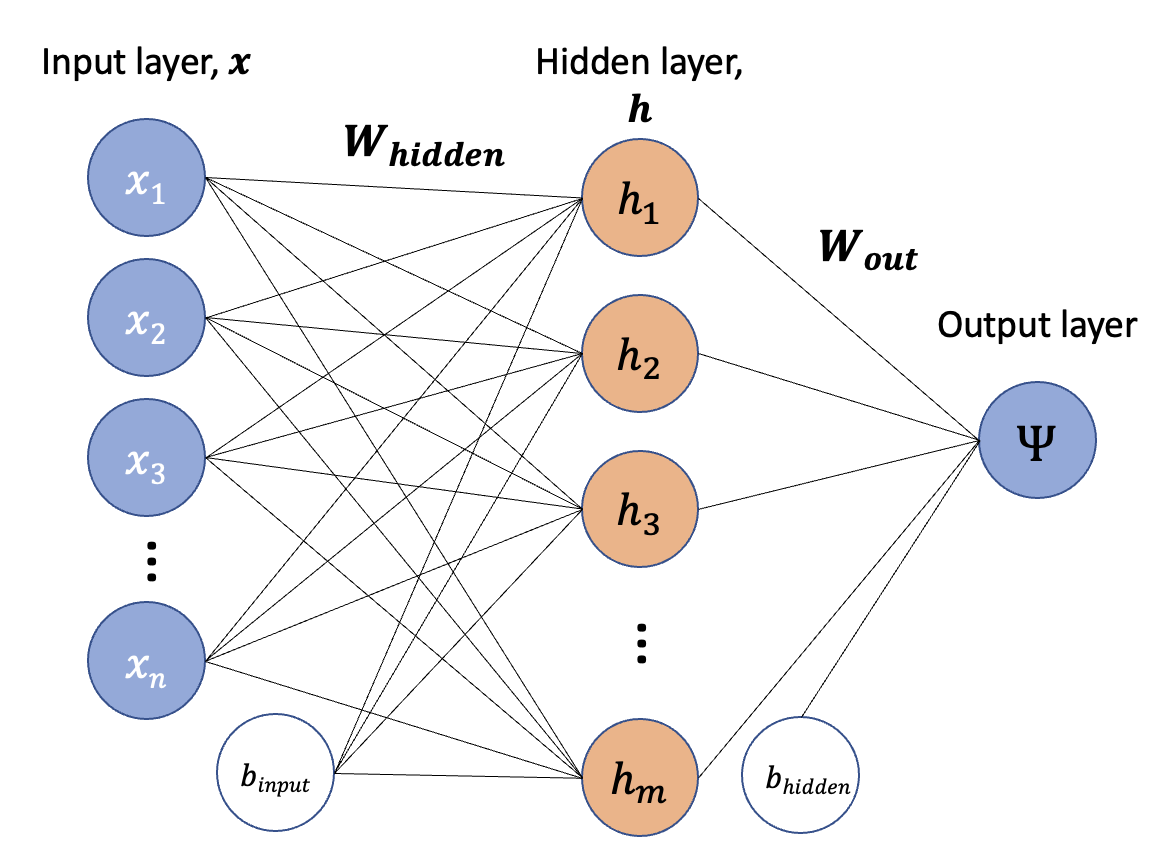
\includegraphics[width=0.6\linewidth]{images/mlp_diagram.png}
    \caption{Structure of a Multilayer Perceptron with one hidden layer and one real-valued output node}
    \label{rbmstructure}
\end{figure}
When approximating the wave function of an Ising model, each input node $x_i$ represents the spin of a particle in the Ising model, and the output nodes represent the value of the wave function. If we assume the wave function to be real and positive, then only one output node is needed to represent the wave function \cite{b20}. With a complex wave function, we could use two output nodes that represent the real and imaginary components of the wave function. With one hidden layer, the MLP representation of the wave function can be expressed as:
\begin{equation}
    \Hat{\Psi}(\boldsymbol{x}; \boldsymbol{\theta}_{mlp}) = 
    \phi_{out} \left(
    \boldsymbol{W}_{out} \hspace{2pt}
    \phi_{hidden} \left( \boldsymbol{W}_{hidden}\boldsymbol{x} + \boldsymbol{b}_{input} \right) + \boldsymbol{b}_{hidden} \right)
\end{equation}
where  $\boldsymbol{\theta}_{mlp} = \{\boldsymbol{W}_{hidden}, \boldsymbol{b}_{input}, \boldsymbol{W}_{out}, \boldsymbol{b}_{hidden}\}$ are the weights and bias of the MLP and $\phi_{hidden}, \phi_{out}$ are the activation functions of the hidden and output layer respectively \cite{b20}. The MLP is trained similarly to the RBM, except a more general sampling method, the Metropolis-Hasting algorithm, is used \cite{b25}.

\section{Hybrid quantum-classical}
Hybrid quantum-classical methods are designed to use current limited quantum computing resources by integrating them with classical optimisers to solve QUBO problems \cite{b32}. One such method is the Quantum Approximate Optimization Algorithm (QAOA), which was first introduced by \outcite{b23}. Like NNQS, QAOA aims to find an approximation of the ground state of the problem Hamiltonian using a gate-based quantum circuit.

QAOA can be regarded as a discretised version of quantum annealing \cite{qaoareview} and consists of repeated applications of the problem Hamiltonian and a mixing Hamiltonian. The one-qubit operations of the problem Hamiltonian are implemented with $R_Z$ rotation gates while the two-qubit operations are implemented with a 2-qubit $R_{ZZ}$ gate. The usual choice of mixing Hamiltonian is the Pauli-X operator acting on each qubit and is implemented with $R_X$ rotation gates. The Hamiltonians are applied repeatedly for time intervals of $\boldsymbol{\gamma}$ and $\boldsymbol{\beta}$ which are variational parameters to be optimised. The algorithm also has a hyperparameter $p$ which decides the number of variational parameters. A circuit diagram of the QAOA circuit is shown in \autoref{qiskitcircuit}. 
\begin{figure}[htb!]
    \centering
    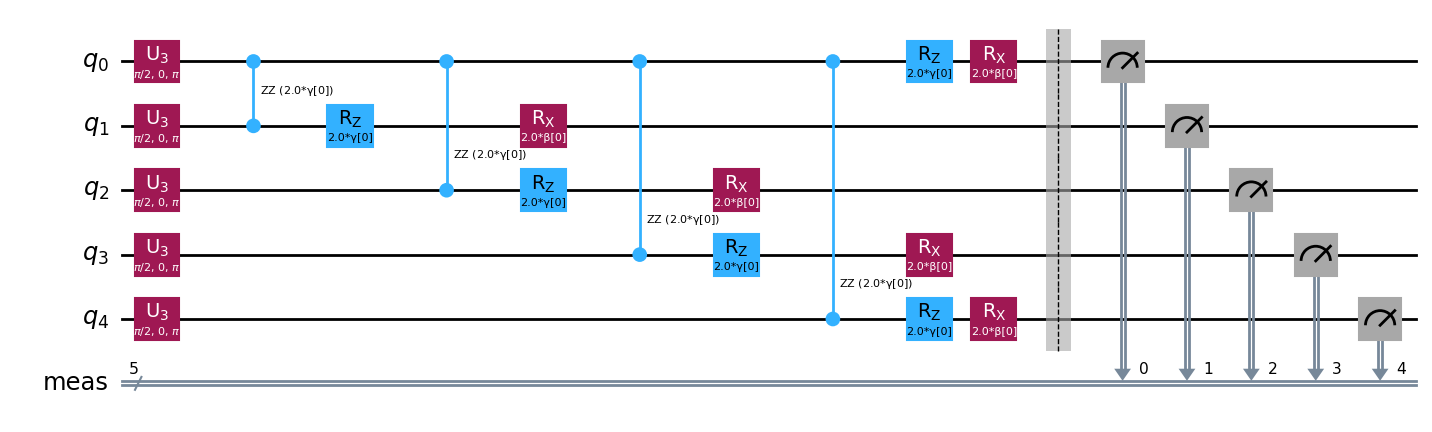
\includegraphics[width=\linewidth]{images/qaoanewcircuit.png}
    \caption{Circuit diagram of the QAOA algorithm circuit with $p=1$. The Hadamard gates on the left put the qubits in a superposition state, followed by the parametrised gates used for the problem (blue) and mixing (red) Hamiltonian, followed by measurements of the qubit states.}
    \label{qiskitcircuit}
\end{figure}

The circuit is measured repeatedly to obtain samples of the qubit configurations that are used to calculate the expected energy, which is minimised by varying $\boldsymbol{\gamma}$ and $\boldsymbol{\beta}$. The final solution is determined by repeated sampling from the optimised circuit.
%\begin{figure}[htb!]
%    \centering
%    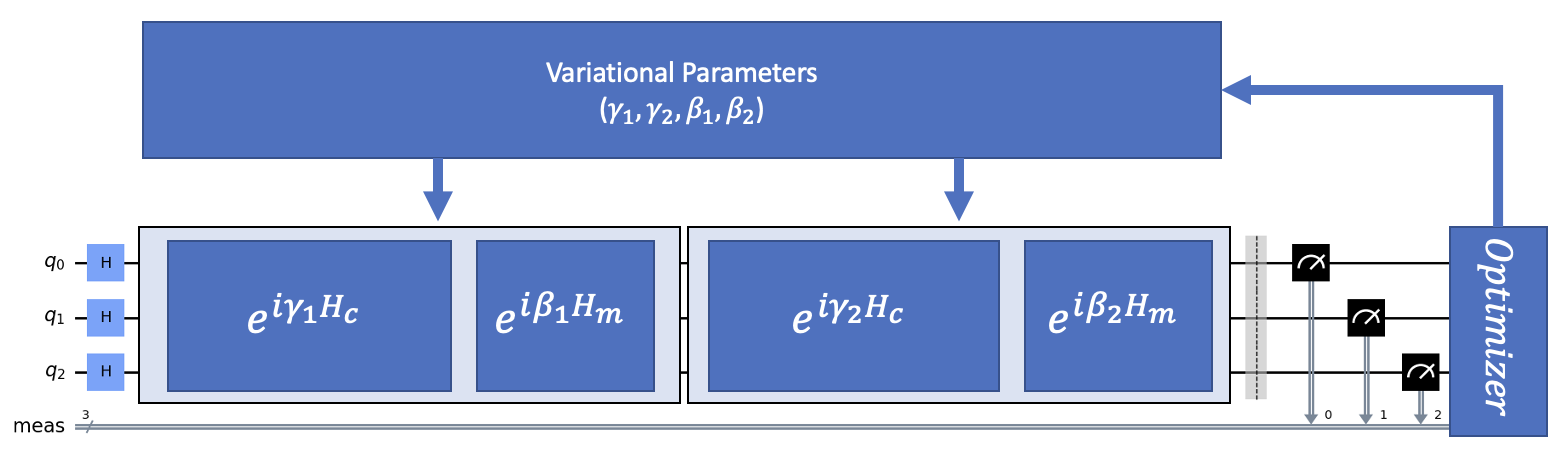
\includegraphics[width=\linewidth]{images/qaoa_circuit.png}
%    \caption{Circuit diagram of the QAOA algorithm circuit with $p=1$}
%    \label{qaoacircuit}
%\end{figure}

In contrast to quantum annealing, which can only be run on specialised quantum annealing devices, QAOA can be implemented on a general gate-based quantum computer \abbrevcite{b22}. In the noisy intermediate-scale quantum (NISQ) era, quantum computers are not yet stable enough to reliably run deep and complex quantum circuits and hybrid methods could serve as the intermediate solution for solving optimisation problems on quantum computers \cite{qaoareview}. Currently, quantum computers can be accessed through service providers such as IBM Quantum and Entropica Labs. There are also many variants of possible QAOA Ansatz and training procedures which are detailed in the review paper by \outcite{qaoareview}.